Das Messverfahren nach Clément-Desormes wurde schon ausreichend erklärt, bei Rüchardt lässt sich nur sagen: Der Druck \(p\) der Gasflasche wurde durch Öffnen des Ventils so lange erhöht und leicht variiert, bis sich eine konstante Oszillation eingestellt hat. Somit konnte mit der Start der Periodendauermessung begonnen werden. 
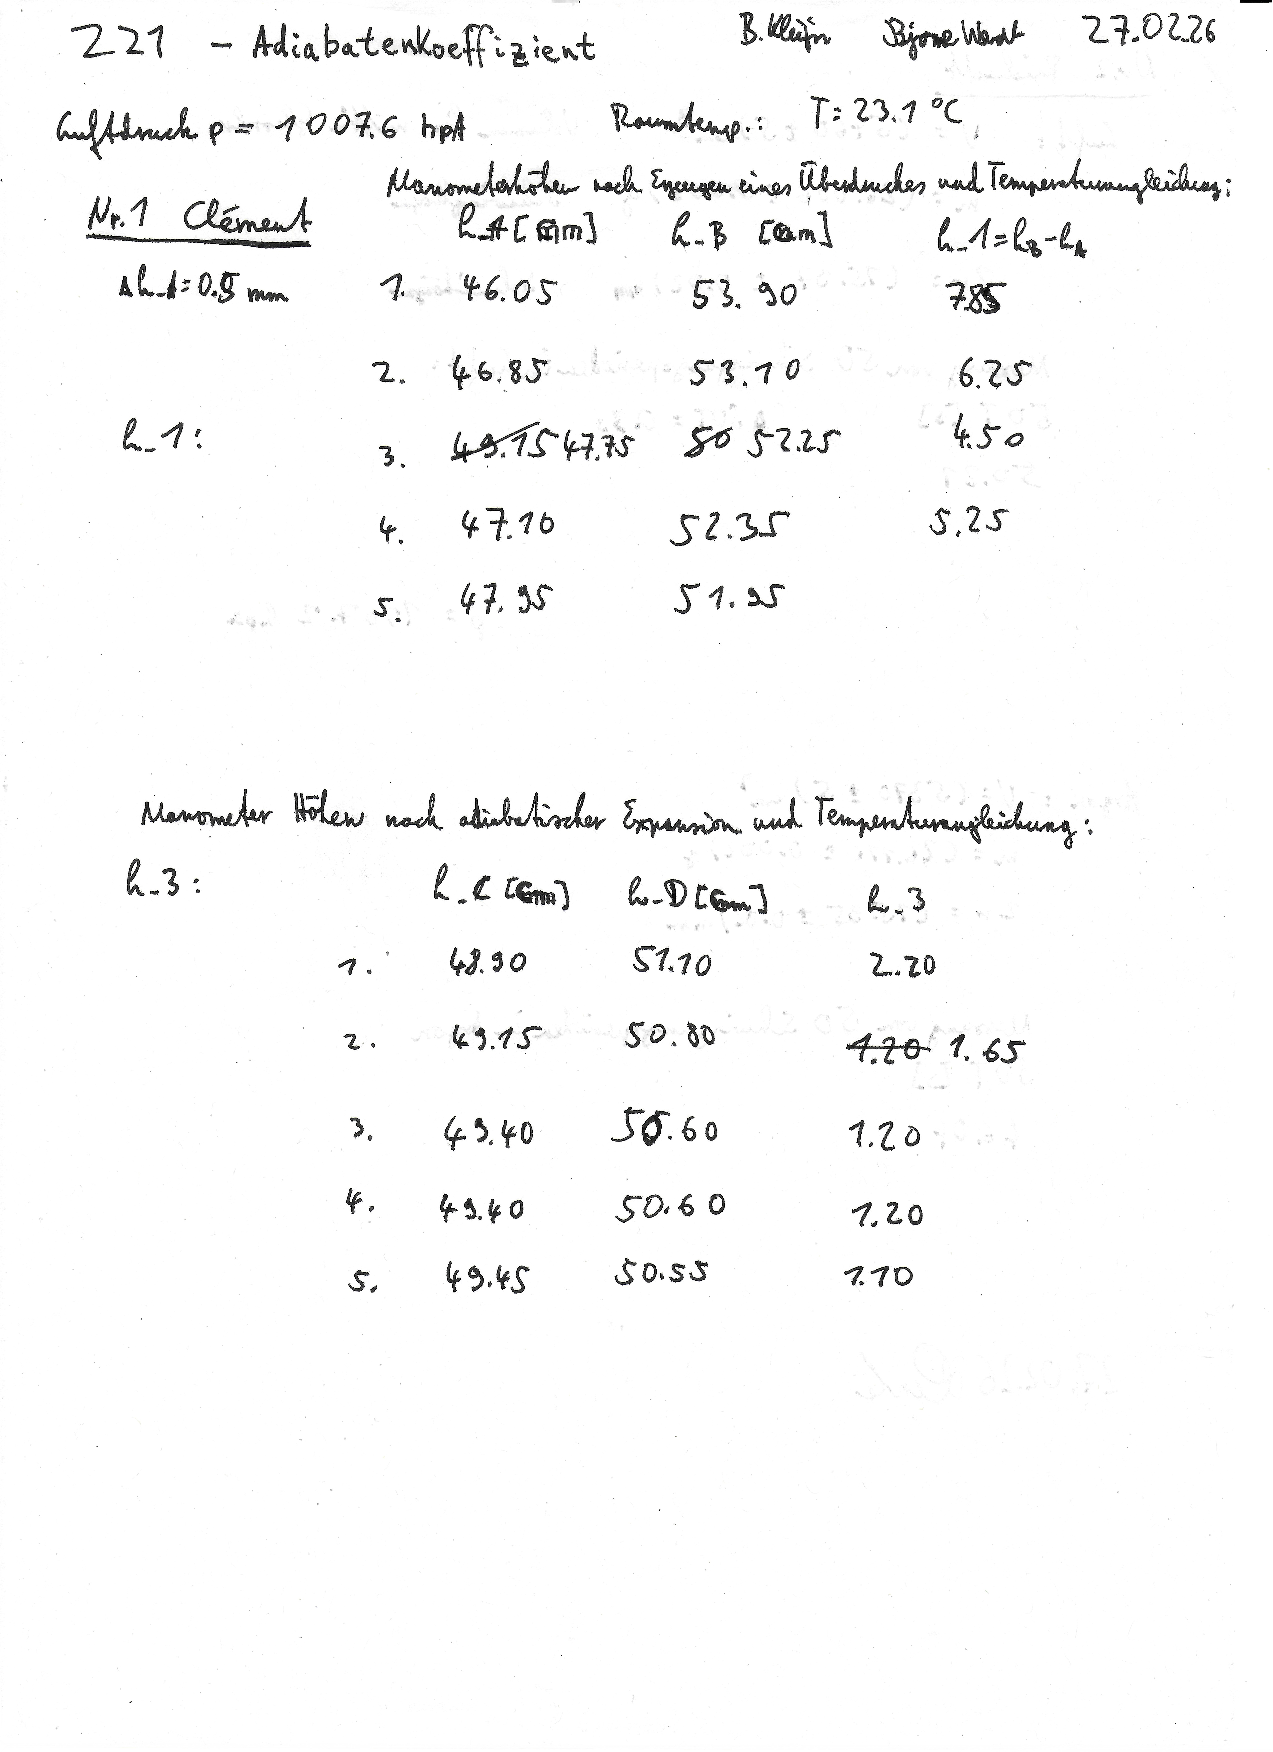
\includepdf[pages=-]{./images/221_Messprotokoll}
